\documentclass[tikz,border=8pt]{standalone}
\usepackage{amsmath,amssymb}
\usetikzlibrary{arrows.meta,automata,positioning,quotes}
\begin{document}
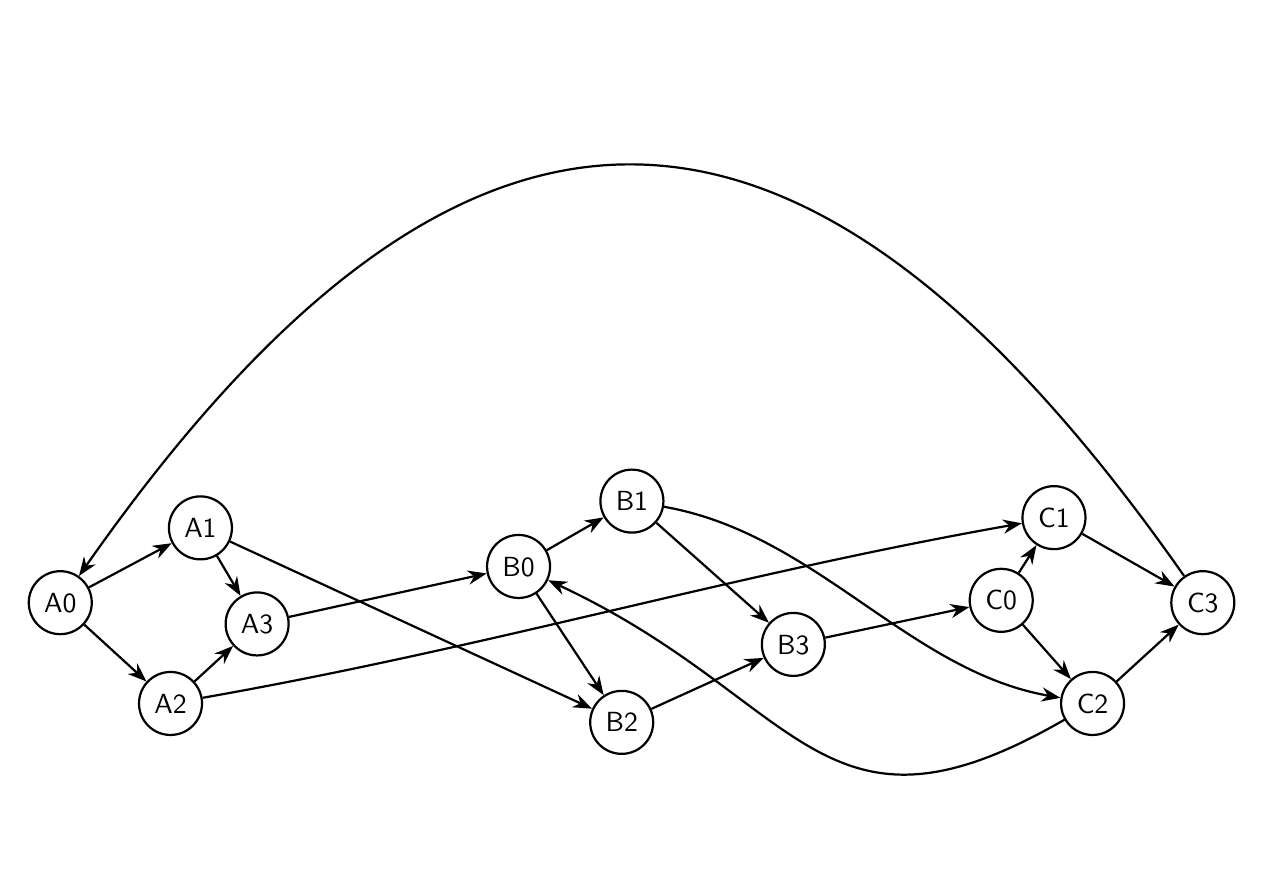
\begin{tikzpicture}[x=1cm,y=1cm]
\tikzset{
  graphnode/.style={circle,draw,thick,minimum size=8mm,inner sep=1pt,font=\sffamily},
  directed/.style={-{Stealth[length=2.4mm]},thick},
  undirected/.style={thick}
}
\node[graphnode] (n_A0) at (-1.06,0.01) {A0};
\node[graphnode] (n_A1) at (0.72,0.96) {A1};
\node[graphnode] (n_A2) at (0.34,-1.27) {A2};
\node[graphnode] (n_A3) at (1.44,-0.26) {A3};
\node[graphnode] (n_B0) at (4.76,0.47) {B0};
\node[graphnode] (n_B1) at (6.20,1.30) {B1};
\node[graphnode] (n_B2) at (6.07,-1.51) {B2};
\node[graphnode] (n_B3) at (8.25,-0.52) {B3};
\node[graphnode] (n_C0) at (10.89,0.04) {C0};
\node[graphnode] (n_C1) at (11.56,1.09) {C1};
\node[graphnode] (n_C2) at (12.05,-1.27) {C2};
\node[graphnode] (n_C3) at (13.45,0.01) {C3};
\draw[directed] (n_A0) -- (n_A1);
\draw[directed] (n_A0) -- (n_A2);
\draw[directed] (n_A1) -- (n_A3);
\draw[directed] (n_A2) -- (n_A3);
\draw[directed] (n_B0) -- (n_B1);
\draw[directed] (n_B0) -- (n_B2);
\draw[directed] (n_B1) -- (n_B3);
\draw[directed] (n_B2) -- (n_B3);
\draw[directed] (n_C0) -- (n_C1);
\draw[directed] (n_C0) -- (n_C2);
\draw[directed] (n_C1) -- (n_C3);
\draw[directed] (n_C2) -- (n_C3);
\draw[directed] (n_A3) -- (n_B0);
\draw[directed] (n_B3) -- (n_C0);
\draw[directed] (n_A1) -- (n_B2);
\draw[directed] (n_A2) to[out=10,in=190,looseness=0.9] (n_C1);
\draw[directed] (n_B1) to[out=-10,in=170,looseness=0.9] (n_C2);
\draw[directed] (n_C3) to[out=125,in=55,looseness=1.55,dashed] (n_A0);
\draw[directed] (n_C2) to[out=-150,in=-25,looseness=1.35,dashed] (n_B0);
\end{tikzpicture}
\end{document}
